\chapter{Preliminaries}
This section covers the knowledge needed in code-clone management, branching management and Git conflicts. It also brings up related work and discusses how this study differs from them.

\section{Code-Clone Management}
Cloning happens during all stages of a software-development process, and it is the responsibility of the developers themselves to make sure that changes between copies of the clones are propagated correctly [1]. Because of this, there are risks that conflicts arise during all stages of the development process. When cloning features, multiple versions of the same feature exists and their consistency needs to be managed [3].

With the use of a version control system, cloning can be managed in a more smooth way by using branching and merging capabilities [3]. \textit{Git} is a fully distributed version control system. It stores the whole project along with a complete development history in a so called \textit{repository}, and since it is fully distributed, one has instant access to the repository. Often when using Git, a remote hosting server is used. \textit{GitHub} is a popular remote hosting server. It has a request limit of 5000 requests per hour, but once a project is cloned, no request limits on project hosting sites are a problem anymore. This makes analyzing a Git-hosted project attractive.

\section{Branching Management}
Many software projects follow a branching model when using Git, such as the one explained by Giessen [4]. In these models, users create feature branches that provide an environment where new features can be implemented and tested without affecting the end-user version of the software [5]. There are various ways to use branches. A branch can be created for each new feature, in this document called \textit{feature-branching}. A branch may also be created for each new product that is to be developed, or each variant of an existing product. Such a branch is in this document called \textit{variance-related branching} [1], for example, for supporting new hardware in an existing product.

When a new feature has been implemented in a new branch, the branch needs to be merged into another branch, such as the main branch. \textit{Merging} is the process of joining two branches together, both in case of two local branches or a local and a remote branch [6]. Local branches are branches in the client’s copy of the repository, whereas the remote branches are branches in the remote repository. In GitHub, merging is usually done using a pull request. A \textit{pull request} is made to let the collaborators in the repository know that the commits in a branch are ready to be merged. The collaborators can review the new code and input their feedback until it is finally approved for merging into the end-user branch [7].
\FloatBarrier
The two commits that are to be merged are called the \textit{parents} of the textit{merge commit} that is created when the merge is made. In this document, the parents will often be referred to as the left- and the right version. The \textit{left version} is the commit that was checked out at the time of the merge, and the \textit{right version} is the commit that is being merged into the currently checked out branch. For instance, when pulling the remote branch to merge with the local branch, the left version will be the local version and the right version will be the remote version that is being pulled. The commit that two branches originates from is called the \textit{common ancestor}. Figure \ref{fig:merging} illustrates a merge and the terms common ancestor, left- and right version, and merge commit.

\begin{figure}[H]
\centering
%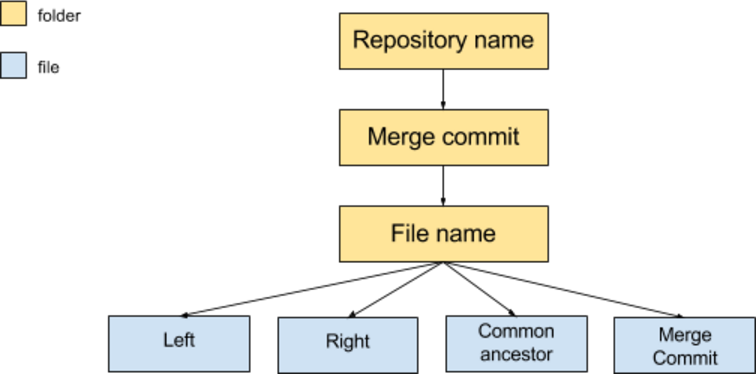
\includegraphics[width=0.45\linewidth, trim=3cm 11cm 3cm 11cm]{figure/conflicts.png}
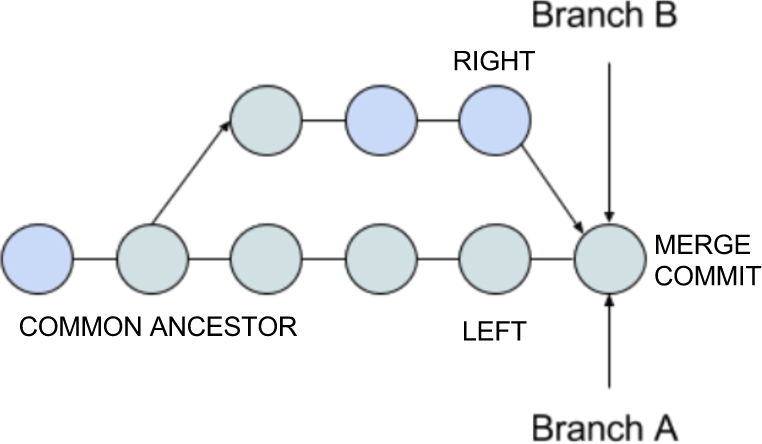
\includegraphics[width=400pt]{figure/merge.png}
\caption{Merging of two branches}\label{fig:merging}
\end{figure}
\FloatBarrier
\textbf{Textual Merging.} The most commonly used merging technique is textual merging [8]. \textit{Textual merging} is based on the history and on textual differences. It does not make use of any knowledge of the syntax or semantic. One must also distinguish between two-way merging and three-way merging. In \textit{two-way merging}, only the two conflicting clones are analyzed to resolve the conflict. In \textit{three-way merging}, also the common ancestor is used, which is more powerful [9].

\textbf{Fast-Forward.} When merging two branches, Git first attempts to perform a so-called fast-forward merge. \textit{Fast-forward} is a way of simplifying merges in cases where at least one of the branches still points to the common ancestor. Since only one version has changed, there can not be any conflicts when merging. In such a case, all that has to be done, is to change both branches to point at the latest commit, as shown in Figure \ref{fig:fastforward}.
\begin{figure}[H]
\centering
\begin{subfigure}[b]{0.3\textwidth}
   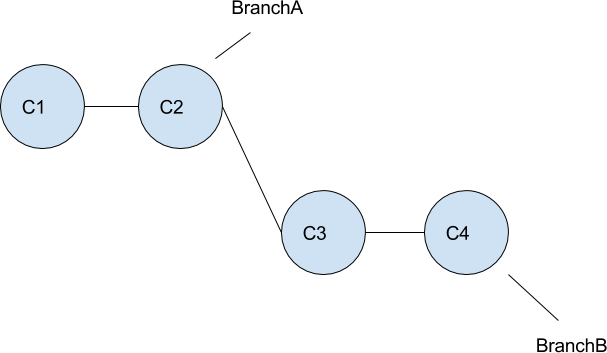
\includegraphics[width=150pt]{figure/ff1.png}
   \caption{Before merge}
   \label{fig:fbranch1}
\end{subfigure}
\begin{subfigure}[b]{0.3\textwidth}
   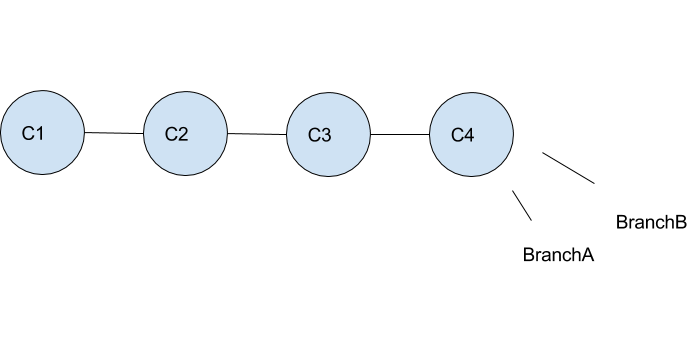
\includegraphics[width=150pt]{figure/ff2.png}
   \caption{After merge}
   \label{fig:fbranch3}
\end{subfigure}
\caption{Fast-forward merge}\label{fig:fastforward}
\end{figure}

\textbf{Three-Way Merge.} If fast forward fails, that is, when commits have been made to both branches that are to be merged, Git has to merge all files that the commits contain. This consists of merging the two versions of every file separately. To be able to know what has changed in the two branches, Git considers both the two versions and their common ancestor. If the files have not been changed at the same places in both branches, Git is able to do this automatically.

\section{Resolving Git Conflicts}
When branches are to be merged in Git, conflicts might arise. \textit{Conflicts} are the problems that prevent Git from automatically merging two branches together. This happens when the two parent commits have made changes to the same place in a file. Resolving conflicts is usually done by manually merging the conflicting lines of the two versions. To do this, one also takes the common ancestor’s version of the file into consideration. By looking at the common ancestor and the two versions, it becomes clear which lines each version has added, and the developer can then choose parts from the two versions. He can choose one version completely, choose parts from both versions and he can add or remove code.

\section{Related Work}

\subsection{Semistructured Merge}
There exist merge tools that use approaches other than textual merging, such as syntactic- and semantic merging, which have language specific knowledge [10] and do not only compare lines of text. A combination of both textual merging, syntactic and semantic merging is called semistructured merging [8]. Studies have shown that the use of semistructured merge decreases the number of conflicts significantly. Cavalcanti et al. prove, by performing semistructured merging on 3266 merge scenarios on 60 projects, that semistructured merging can reduce the number of conflicts by 55\% [11]. Our work is different in that instead of proposing a new conflict resolution technique, we are interested in how developers resolve conflicts arising from different variants of features or projects.

\subsection{Conflict Patterns}\label{sec:cp}
During merging, several types of conflict patterns might occur. Previous work by Accioly [12] identified numerous conflict patterns, using her developed tool Conflicts Analyzer.

In her study, Accioly lists conflict patterns that describe types of conflicts that might arise during a merge. The study uses a semi-structured merge tool, called SSMerge, which performs merges by first constructing Feature-Structured Trees (FSTs) for the two versions of the file that are to be merged. The two trees are then merged using superimposition. This is possible since the order of methods and class variables inside a class does not matter. Code segments where the ordering matters in Java, ie. method- and constructor bodies, cannot be merged this way and are therefore placed in the leaves of the tree [8]. It is the conflicts that concern these leaves that are of interest to our study. We will use Conflicts Analyzer and the conflict patterns to analyze and categorize merge-conflict resolutions.


The conflict patterns are derived from the conflicts that SSMerge can detect [12]. Table \ref{table:conflictpatterns} lists the patterns from Accioly’s study that is listed in the online appendix:\\% HELLO FERRET, INSERT FOOT NOTE FROM THESIS REKÅT
\begin{table}
\caption{Conflict patterns}\label{table:conflictpatterns}
\begin{tabular}{| l | p{10cm} |}
\hline
\multicolumn{1}{c}{\textbf{Pattern}} & \multicolumn{1}{c}{\textbf{Description}}\\
EditSameMC & Different edits to the same area of the same method or constructor\\
SameSignatureCM & Methods or constructors added with the same signature and different bodies\\
EditSameFd & Different edits to the same field declaration\\
AddSameFd & Field declarations added with the same identifiers and different types of modifiers\\
ModifierList & Different edits to the modifier list of the same type declaration (class, interface, annotation or enum types)\\
ImplementsList & Different edits to the same implements declaration\\
ExtendsList & Different edits to the same extends declaration\\
DefaultValueA & Different edits to the same annotation method default value
\end{tabular}
\end{table}
From Table \ref{table:conflictpatterns}, it is the EditSameMC- and SameSignatureCM patterns that concern the leaves of the tree.

\subsection{Avoiding Software Merge-Conflicts}
There exist numerous practices to reduce merge-conflicts, such as continuous integration[13] in an Agile development process. The continuous integration practice makes sure that developers merge their code in short intervals and therefore the conflicts does not become as many at a given time as it would if merges were done less frequently.

Furthermore, Guimaraes and Silva[14] argues that developers do not merge as frequently as desirable. They state that “\textit{Unfortunately, merging is cumbersome and disrupts programming flow, so some developers do not merge as frequently as desirable — teams avoid parallel work because of difficult merges, and developers rush their tasks to avoid being the ones responsible for the merge.}” To aid developers when merging, they present a solution that continuously merges committed and uncommitted code in the background, and then presents detected conflicts to the developer inside the IDE, while the developer continues developing.

While Guimaraes and Silva strive to avoid conflicts, our long term goal is to ease the solving of merge-conflicts by automatically solving them using a tool. This study will contribute to the long term goal by analyzing and categorizing merge-conflict resolutions done by real developers.

\subsection{Variance in Code-Clone Management}
Dubinsky et. al. [1] have conducted an exploratory study of cloning in industrial software product lines. In their study, they state that it is difficult to propagate changes between clones. They have also interviewed developers who say that “\textit{If we find a bug then many times it can be here and also in other places. The new product contains code that exists also in the old product. So, if we fix the old one then we also fix the new or vice versa}”. Moreover, they say that sometimes they find the same bug in different variants which nobody thought about before.

We believe that our study can build on Dubinsky et. al’s. study by answering RQ1. Identifying variance-related branches will ease the process of propagating changes between clones in an industrial software product line since the developers would know which branches they should propagate.